% Draft for IEEE Access. Written with the standard IEEEtran journal class so it compiles with a
% stock TeX Live; to submit, move the content into the official IEEE Access template
% (ieeeaccess.cls from the IEEE Author Center) -- see paper/README.md.
\documentclass[journal]{IEEEtran}

\usepackage{amsmath,amssymb}
\usepackage{graphicx}
\usepackage{booktabs}
\usepackage{multirow}
\usepackage{siunitx}
\usepackage{xcolor}
\usepackage{tikz}
\usetikzlibrary{arrows.meta,positioning,fit,calc,backgrounds}
\usepackage[hidelinks]{hyperref}
\usepackage{cite}

\newcommand{\pmstd}[2]{#1\,{\scriptsize$\pm$#2}}
\graphicspath{{figures/}}

\begin{document}

\title{Lightweight Thermal-to-Visible Face Recognition on the Edge: Adaptation, Forgetting, and Quantization on a License-Free Benchmark}

\author{Ronit~Mittal%
\thanks{R.~Mittal is with the University of Petroleum and Energy Studies (UPES), Dehradun, India (e-mail: ronitmittal0@gmail.com).}}

\markboth{IEEE Access}{Mittal: Lightweight Thermal-to-Visible Face Recognition on the Edge}

\maketitle

\begin{abstract}
Compact face recognition (FR) networks such as EdgeFace approach state-of-the-art accuracy on visible-light benchmarks with fewer than two million parameters, yet the cameras that edge systems rely on at night or in harsh illumination are increasingly thermal, and these networks are rarely evaluated in that band. This paper presents a systematic study of lightweight thermal-to-visible heterogeneous face recognition (HFR) under three constraints that matter on edge devices: few trainable parameters, no loss of visible-light accuracy, and 8-bit integer (INT8) deployment. To keep the study reproducible without data-access agreements, a subject-disjoint, five-fold protocol is built on the openly licensed SpeakingFaces corpus. A pretrained EdgeFace-XS model reaches 100\% visible-to-visible but only 34.0\% thermal-to-visible rank-1 accuracy on this protocol. Eight adaptation strategies are compared over 15 runs each: full fine-tuning, three shared parameter-efficient methods (BitFit, LayerNorm tuning, and LoRA adapted to factorized layers), and four modality-specific methods, including a rank-space modulation of the factorized layers proposed here. Three findings emerge. First, every method that shares parameters with the visible path forgets 0.8--2.0 percentage points (pp) of LFW accuracy, whereas modality-specific LayerNorm matches the rank-1 accuracy of shared LayerNorm tuning (92.1\% vs.\ 92.3\%) with zero visible-light forgetting by construction, at a cost of 6.5\,pp in true accept rate at a false accept rate of 0.1\%. Second, dynamic INT8 quantization is strongly modality-asymmetric: it costs at most 0.3\,pp of visible-to-visible rank-1 accuracy but 2.2--13.7\,pp of thermal-to-visible rank-1 accuracy, and the loss grows as fewer parameters are adapted. Third, this loss originates in the first three of the four stages, mainly in the third: quantizing only the last stage, which holds 51\% of the linear-layer weights, stays within 1.2\,pp of FP32 for every method and is also the fastest quantized configuration on an x86 CPU, where full dynamic INT8 is slower than FP32. The protocol, code, and all per-run results are released.
\end{abstract}

\begin{IEEEkeywords}
Heterogeneous face recognition, thermal imaging, efficient neural networks, parameter-efficient fine-tuning, catastrophic forgetting, post-training quantization, mixed precision, edge computing.
\end{IEEEkeywords}

%=====================================================================
\section{Introduction}
%=====================================================================
\IEEEPARstart{F}{ace} recognition (FR) has moved from the data center to the edge. Compact networks such as MobileFaceNets~\cite{chen2018mobilefacenets} and EdgeFace~\cite{george2024edgeface}, the latter combining the hybrid CNN--Transformer EdgeNeXt~\cite{maaz2022edgenext} with low-rank factorized linear layers, achieve high verification accuracy with a few million parameters and a few hundred million floating-point operations, and efficient-FR challenges~\cite{deng2019lightweight} have made such models a mature research topic. Their evaluation, however, remains almost exclusively visible-light. Many of the places where an edge FR system has to work are not well lit: building access at night, in-cabin driver monitoring, and perimeter surveillance increasingly use long-wave infrared (thermal) cameras, which are insensitive to ambient illumination and harder to deceive with printed photographs~\cite{hermosilla2012thermal}. Enrolment, on the other hand, almost always happens with ordinary visible-light photographs. Matching a thermal probe against a visible gallery is a heterogeneous face recognition (HFR) problem, and a difficult one: a thermal camera records emitted rather than reflected radiation, so texture, hair, and eye regions look fundamentally different (Fig.~\ref{fig:samples}).

HFR has been studied extensively for large networks~\cite{sarfraz2017dpm,wu2018lightcnn,fu2019dvg,george2023pdt}, but three questions that decide whether it is practical on an edge device remain open for lightweight models:
\begin{enumerate}
\item \emph{How should a compact model be adapted to the thermal band?} Storing a fully fine-tuned copy per modality doubles the memory footprint, and parameter-efficient fine-tuning (PEFT) methods~\cite{houlsby2019adapters,benzaken2022bitfit,hu2022lora} were designed for much larger networks than a 1.8\,M-parameter face model.
\item \emph{What happens to the visible-light task?} A deployed model usually has to serve visible probes as well, and adapting it to thermal data can cause catastrophic forgetting~\cite{kirkpatrick2017ewc,li2018lwf}.
\item \emph{What does quantization do to cross-modal matching?} Edge deployment nearly always involves 8-bit integer (INT8) arithmetic~\cite{jacob2018quantization,krishnamoorthi2018whitepaper}, yet quantized FR models are validated on visible-light benchmarks only.
\end{enumerate}

A practical obstacle to answering these questions is data access. The standard cross-spectral face benchmarks, such as CASIA NIR-VIS~2.0~\cite{li2013casia} and the ARL Visible-Thermal Face dataset~\cite{poster2021arlvtf}, are distributed under individual license agreements, which makes it hard for many groups to reproduce or extend published results. This study is therefore built entirely on SpeakingFaces~\cite{abdrakhmanova2021speakingfaces}, a corpus of synchronized and spatially registered thermal and visible video of 142 subjects released under the Creative Commons Attribution 4.0 license, which anyone can download without a request.

\begin{figure}[t]
\centering
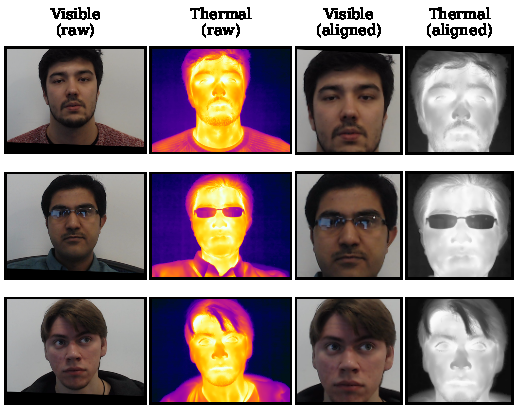
\includegraphics[width=\columnwidth]{dataset_samples.pdf}
\caption{Registered visible and thermal frames from SpeakingFaces~\cite{abdrakhmanova2021speakingfaces} (CC BY 4.0) and the $112\times112$ crops produced by the alignment pipeline (Section~\ref{sec:benchmark}). Thermal frames are rendered in false color by the dataset and converted to gray scale for recognition. Eyeglasses are opaque at thermal wavelengths (middle row), one of the reasons thermal-to-visible matching is hard.}
\label{fig:samples}
\end{figure}

\noindent The contributions of this paper are as follows.
\begin{itemize}
\item \textbf{A reproducible, license-free benchmark} for lightweight thermal-to-visible FR: subject-disjoint five-fold cross-validation with fixed gallery and probe definitions, and a pipeline that downloads only the frames it needs (about 3\,GB instead of the 1.2\,TB release) and aligns both modalities with a single geometric transform.
\item \textbf{A controlled comparison of eight adaptation strategies} for EdgeFace over five folds and three seeds, which measures thermal accuracy and visible-light forgetting jointly. It includes a rank-space modulation (RSM) of factorized layers, introduced here, and shows that normalization parameters, rather than the factorized subspaces, carry most of the modality-specific information.
\item \textbf{Evidence that INT8 quantization is modality-asymmetric for HFR}: it leaves visible matching essentially untouched but costs up to 13.7\,pp of thermal rank-1 accuracy, more so for methods that adapt fewer parameters.
\item \textbf{A stage-wise sensitivity analysis} which traces this loss to the first three stages, mainly the third, and to an erosion of the genuine-score margin, leading to a simple mixed-precision configuration that is within 1.2\,pp of FP32 for every method, together with CPU latency measurements showing that dynamic INT8 does not accelerate these low-rank models on x86 processors.
\end{itemize}

The remainder of the paper is organized as follows. Section~\ref{sec:related} reviews related work. Section~\ref{sec:benchmark} describes the benchmark, Section~\ref{sec:methods} the adaptation and quantization methods, and Section~\ref{sec:setup} the experimental setup. Section~\ref{sec:results} presents the results, Section~\ref{sec:discussion} discusses their implications and limitations, and Section~\ref{sec:conclusion} concludes.

%=====================================================================
\section{Related Work}
\label{sec:related}
%=====================================================================
\subsection{Efficient Face Recognition}
MobileFaceNets~\cite{chen2018mobilefacenets} adapted mobile CNN design to face embeddings, and the Lightweight Face Recognition Challenge~\cite{deng2019lightweight} established common compute budgets for the task. EdgeFace~\cite{george2024edgeface} builds on EdgeNeXt~\cite{maaz2022edgenext}, which combines convolutional encoders with split depth-wise transposed attention, and replaces each linear layer by a low-rank factorization $W=UV$ (LoRaLin), reducing parameters and computation with little loss in accuracy. These models are trained with margin-based softmax losses such as ArcFace~\cite{deng2019arcface} on large visible-light datasets and evaluated on visible-light verification benchmarks such as LFW~\cite{huang2007lfw}. This paper asks how such a model behaves, and how it should be adapted, when the probe is thermal.

\subsection{Heterogeneous and Thermal Face Recognition}
Early thermal FR relied on hand-crafted local descriptors~\cite{hermosilla2012thermal}. Deep HFR methods learn a mapping from thermal to visible features~\cite{sarfraz2017dpm}, learn modality-invariant representations with light-weight backbones~\cite{wu2018lightcnn}, synthesize paired training data with generative models~\cite{fu2019dvg}, or prepend a small modality-specific network to a frozen visible-light FR model, as in the Prepended Domain Transformer~\cite{george2023pdt}. The last design keeps the visible path intact and is closest in spirit to the modality-specific methods studied here. Most of these works use large backbones and evaluate in floating point; edge constraints are rarely considered. Benchmarks with paired thermal and visible faces include ARL-VTF~\cite{poster2021arlvtf}, the Tufts Face Database~\cite{panetta2020tufts}, and SpeakingFaces~\cite{abdrakhmanova2021speakingfaces}; only the last is released under an open license that requires no data-access request.

\subsection{Parameter-Efficient Adaptation and Forgetting}
Adapters~\cite{houlsby2019adapters} insert small trainable modules into a frozen network, BitFit~\cite{benzaken2022bitfit} tunes only bias terms, and LoRA~\cite{hu2022lora} learns low-rank weight updates. Normalization parameters alone are surprisingly expressive~\cite{frankle2021batchnorm}, and re-estimating or separating normalization statistics per domain is an established tool for domain adaptation~\cite{li2018adabn,chang2019dsbn}. Fine-tuning on a new domain can degrade performance on the original one~\cite{kirkpatrick2017ewc}; regularization-based methods such as Learning without Forgetting~\cite{li2018lwf} mitigate this, whereas modality-specific parameters avoid it by construction.

\subsection{Quantization}
Integer quantization~\cite{jacob2018quantization} is the standard way to reduce the size and latency of networks on edge hardware~\cite{krishnamoorthi2018whitepaper,nagel2021whitepaper,gholami2021survey,wu2020integer}. Post-training dynamic quantization stores weights in INT8 and quantizes activations on the fly, requiring no calibration data. Mixed-precision methods assign different bit widths to layers according to their sensitivity~\cite{dong2019hawq}. To the best of our knowledge, the interaction between quantization and cross-modal matching in lightweight HFR has not been characterized.

%=====================================================================
\section{A License-Free Thermal-to-Visible Benchmark}
\label{sec:benchmark}
%=====================================================================
\subsection{Data}
SpeakingFaces~\cite{abdrakhmanova2021speakingfaces} contains synchronized thermal and visible video of 142 subjects reading commands, recorded in two trials per subject at nine head positions, with the visible stream registered pixel by pixel to the $464\times348$ thermal stream. One subject (ID~2) has no image data in the public release, leaving 141 subjects. For every subject, trial, and position, frames 100, 300, 500, and 700 of the 900-frame clip are used, yielding 72 thermal--visible pairs per subject. Because the archives total about 1.2\,TB, the pipeline reads only the required files from the remote archives with HTTP range requests. Table~\ref{tab:data} summarizes the resulting data, and Fig.~\ref{fig:poses} shows the nine head positions.

\begin{table}[t]
\centering
\caption{Benchmark Statistics}
\label{tab:data}
\begin{tabular}{lr}
\toprule
Subjects with image data & 141 \\
Trials $\times$ head positions $\times$ frames per subject & $2\times9\times4$ \\
Thermal--visible pairs (aligned / total) & 10{,}101 / 10{,}152 \\
Training subjects per fold & 112--113 \\
Test subjects (gallery templates) per fold & 28--29 \\
Thermal probes per fold & 1{,}000--1{,}039 \\
Probe--template pairs per fold & ${\approx}$28{,}000 \\
Downloaded data & ${\approx}$3\,GB \\
License & CC BY 4.0 \\
\bottomrule
\end{tabular}
\end{table}

\begin{figure*}[t]
\centering
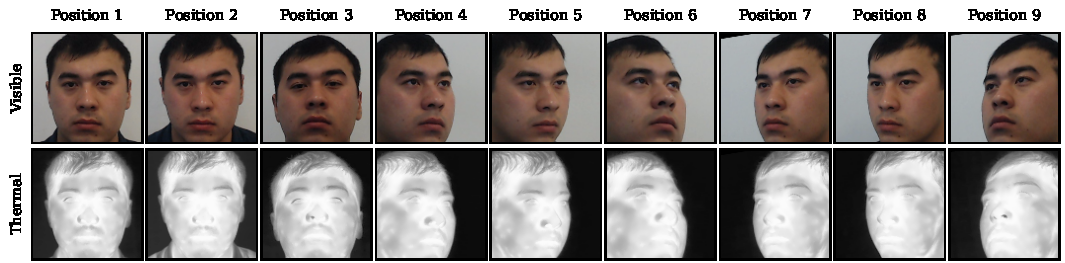
\includegraphics[width=\textwidth]{poses.pdf}
\caption{Aligned visible (top) and thermal (bottom) crops of one SpeakingFaces subject at the nine head positions (trial 2). Position 1 is frontal; the gallery uses frontal visible images of trial 1, and thermal probes are taken from all positions of trial 2.}
\label{fig:poses}
\end{figure*}

\subsection{Alignment}
Five facial landmarks are detected with MTCNN~\cite{zhang2016mtcnn} on the visible frame, a similarity transform to the standard $112\times112$ ArcFace template is estimated, and the \emph{same} transform is applied to the registered thermal frame. Landmark detection on thermal images is unreliable, and this shared transform guarantees that both crops cover exactly the same facial region. Detection failed for 51 of the 10{,}152 pairs (0.5\%), which are discarded. The false-color thermal rendering is converted to gray scale and replicated over three channels.

\subsection{Protocol}
Subjects are assigned to five folds by subject ID ($\text{ID} \bmod 5$). For each fold, the remaining subjects form the training set, and the test set is defined as follows.
\begin{itemize}
\item \textbf{Gallery}: visible images of trial~1 at the frontal position, averaged into one L2-normalized template per subject.
\item \textbf{Probes}: thermal images of trial~2 at all nine positions. Trial~2 is a separate recording, so probes never share frames with the gallery.
\item \textbf{Identification}: closed-set rank-1 accuracy.
\item \textbf{Verification}: all probe--template pairs, reported as the true accept rate (TAR) at a false accept rate (FAR) of $10^{-3}$, and the equal error rate (EER).
\item \textbf{Visible sanity check}: the same protocol with visible probes (VIS$\to$VIS).
\item \textbf{Forgetting}: LFW~\cite{huang2007lfw} verification accuracy of the adapted model's visible path, using the standard 10-fold protocol.
\end{itemize}
Every method is trained on each of the five training sets with three seeds, and results are reported as the mean $\pm$ standard deviation over the 15 runs. Because the folds differ in difficulty, the standard deviation mostly reflects fold-to-fold variation; when two methods are compared, paired differences over the same fold and seed are also reported.

%=====================================================================
\section{Adaptation and Quantization Methods}
\label{sec:methods}
%=====================================================================
\subsection{Backbone}
All methods start from the public EdgeFace-XS ($\gamma=0.6$) checkpoint~\cite{george2024edgeface}. It has 1.77\,M parameters, four EdgeNeXt stages, and 43 factorized layers
\begin{equation}
y = U V x + b, \qquad U\in\mathbb{R}^{d_o\times r},\; V\in\mathbb{R}^{r\times d_i},
\end{equation}
whose rank $r$ is a fraction $\gamma$ of $\min(d_i, d_o)$. Its normalization layers are LayerNorms (21 channel-last and 5 channel-first). Training mixes thermal and visible images of the training subjects, with an ArcFace classification head that is discarded after training.

\subsection{Shared Adaptation}
These methods update parameters that both modalities use.
\begin{itemize}
\item \emph{Full fine-tuning} trains all 1.77\,M weights.
\item \emph{BitFit}~\cite{benzaken2022bitfit} trains the 15{,}400 bias parameters.
\item \emph{LN tuning} trains the affine parameters of all LayerNorms (5{,}080 parameters).
\item \emph{LoRA}~\cite{hu2022lora} cannot be added to a factorized layer without changing its form, so it is implemented as a rank expansion,
\begin{equation}
y = \begin{bmatrix} U & B \end{bmatrix} \begin{bmatrix} V \\ A \end{bmatrix} x + b = UVx + BAx + b,
\end{equation}
with $A\in\mathbb{R}^{k\times d_i}$ randomly initialized, $B\in\mathbb{R}^{d_o\times k}$ initialized to zero, and only $A$ and $B$ trained. With $k=1$ this adds 20{,}480 parameters. The result is again a factorized layer of rank $r+k$, so quantized export is unchanged.
\end{itemize}

\subsection{Modality-Specific Adaptation}
These methods keep separate parameters for each modality $m\in\{\text{vis},\text{thr}\}$, freeze the backbone, and fix the visible copy at its pretrained value, so that the visible path is \emph{exactly} the pretrained network and visible accuracy cannot change. The modality of an input is known at inference time from the camera that captured it. Fig.~\ref{fig:method} illustrates both methods.

\begin{figure}[t]
\centering
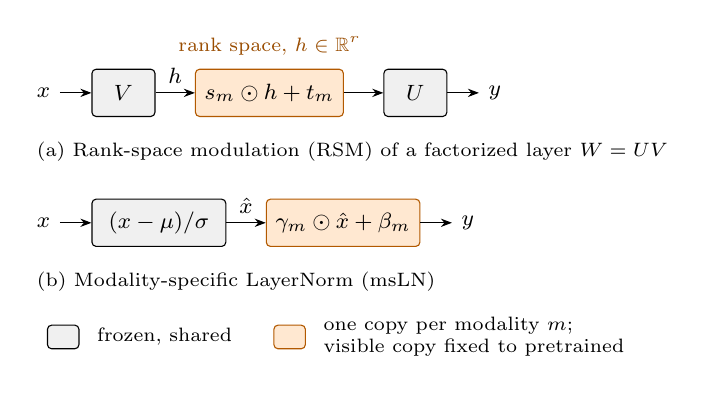
\begin{tikzpicture}[
  font=\footnotesize, >={Stealth[length=4pt]},
  blk/.style={draw, rounded corners=1.5pt, minimum height=6mm, minimum width=8mm, align=center, fill=white},
  frz/.style={blk, fill=gray!12},
  mod/.style={blk, fill=orange!18, draw=orange!70!black},
]
% factorized layer with rank-space modulation
\node (x) {$x$};
\node[frz, right=4mm of x] (V) {$V$};
\node[mod, right=5mm of V, minimum width=17mm] (m) {$s_m\odot h + t_m$};
\node[frz, right=5mm of m] (U) {$U$};
\node[right=4mm of U] (y) {$y$};
\draw[->] (x) -- (V);
\draw[->] (V) -- node[above]{$h$} (m);
\draw[->] (m) -- (U);
\draw[->] (U) -- (y);
\node[above=0.5mm of m, font=\scriptsize, text=orange!60!black] {rank space, $h\in\mathbb{R}^{r}$};
\node[font=\scriptsize, anchor=west] at ($(x.west)+(0,-0.75)$) {(a) Rank-space modulation (RSM) of a factorized layer $W=UV$};
% layernorm
\node (x2) at ($(x)+(0,-1.65)$) {$x$};
\node[frz, right=4mm of x2, minimum width=17mm] (n) {$(x-\mu)/\sigma$};
\node[mod, right=5mm of n, minimum width=17mm] (a) {$\gamma_m\odot\hat{x}+\beta_m$};
\node[right=4mm of a] (y2) {$y$};
\draw[->] (x2) -- (n);
\draw[->] (n) -- node[above]{$\hat{x}$} (a);
\draw[->] (a) -- (y2);
\node[font=\scriptsize, anchor=west] at ($(x2.west)+(0,-0.75)$) {(b) Modality-specific LayerNorm (msLN)};
% legend
\node[frz, minimum width=4mm, minimum height=3mm] (l1) at ($(x2)+(0.25,-1.45)$) {};
\node[right=1mm of l1, font=\scriptsize] (t1) {frozen, shared};
\node[mod, minimum width=4mm, minimum height=3mm, right=4mm of t1] (l2) {};
\node[right=1mm of l2, font=\scriptsize, align=left] {one copy per modality $m$;\\ visible copy fixed to pretrained};
\end{tikzpicture}
\caption{Modality-specific adaptation. Gray blocks are pretrained and shared; orange blocks hold one parameter vector per modality, selected by the input's modality. Fixing the visible copy to its pretrained value ($s=\mathbf{1}$, $t=\mathbf{0}$, pretrained $\gamma,\beta$) makes the visible path identical to the pretrained network. For a fixed modality, both operations fold into the adjacent weights, so inference costs nothing extra.}
\label{fig:method}
\end{figure}

\emph{Modality-specific LayerNorm} (msLN) follows the idea of domain-specific normalization~\cite{chang2019dsbn}: each LayerNorm keeps one pair of affine parameters per modality,
\begin{equation}
y = \gamma_m \odot \frac{x-\mu(x)}{\sigma(x)} + \beta_m,
\end{equation}
which adds 5{,}080 thermal parameters.

\emph{Rank-space modulation} (RSM), proposed here, exploits the structure of EdgeFace. Each factorized layer passes its input through an $r$-dimensional bottleneck $h=Vx$, which is a natural, low-dimensional place to inject modality information:
\begin{equation}
y = U\big(s_m \odot Vx + t_m\big) + b,
\end{equation}
with per-modality scale $s_m\in\mathbb{R}^r$ (initialized to ones) and shift $t_m\in\mathbb{R}^r$ (initialized to zeros). For a fixed modality, $s_m$ folds into $U$ and $U t_m$ into $b$. Three variants are evaluated: the scale only (\emph{RSM-s}, 2{,}653 thermal parameters), scale and shift (\emph{RSM}, 5{,}306 parameters), and RSM combined with msLN (\emph{RSM+msLN}, 10{,}386 parameters).

\subsection{Quantization}
Models are quantized with PyTorch post-training dynamic quantization of all linear layers (the fbgemm backend), which is the standard INT8 path for transformer-style models on CPUs. Weights are quantized per tensor and symmetrically,
\begin{equation}
w_q = \operatorname{clamp}\!\big(\lfloor w/\Delta_w \rceil, -128, 127\big), \quad \Delta_w = \max|w|/127.5,
\end{equation}
and each input activation tensor is quantized at run time, asymmetrically, to the reduced range $[0,127]$ that the x86 kernels use to avoid overflow,
\begin{equation}
\begin{gathered}
x_q = \operatorname{clamp}\!\big(\lfloor x/\Delta_x \rceil + z, 0, 127\big),\\
\Delta_x = \frac{x_{\max}-x_{\min}}{127},\qquad z = \lfloor -x_{\min}/\Delta_x \rceil,
\end{gathered}
\end{equation}
where $x_{\min}\le0\le x_{\max}$ are the tensor's extremes. Convolutions and normalization layers remain in FP32. \emph{Mixed-precision} variants quantize only the linear layers of a chosen subset of the four stages. In this model, stages 1--4 hold 1.2\%, 5.7\%, 37.0\%, and 50.9\% of the 1.57\,M linear-layer weights, respectively, and the embedding head holds the remaining 5.2\%, which stays in FP32 in the mixed-precision variants.

%=====================================================================
\section{Experimental Setup}
\label{sec:setup}
%=====================================================================
All models are trained for 20 epochs with batch size 128, AdamW, a one-cycle learning-rate schedule with 10\% warm-up, and the ArcFace loss (scale 64, margin 0.5). The ArcFace head uses a learning rate of $10^{-2}$. Full fine-tuning uses $10^{-4}$ and a weight decay of 0.05; BitFit, LN tuning, LoRA, and msLN use $10^{-3}$; and RSM vectors use $10^{-2}$; the adapted parameters of the parameter-efficient methods have no weight decay. Horizontal flipping is the only augmentation. For each method, the learning rate was chosen from two candidates on a development split (training subjects 1--80, validation subjects 81--100) with the same budget for every method. Training one model takes 3--5 minutes on one NVIDIA H100 GPU. INT8 models are evaluated on CPU, since the dynamic INT8 kernels are CPU-only. Latency is measured with PyTorch~2.4 on an Intel Xeon Platinum 8470 CPU, for single $112\times112$ images, as the median of 200 runs after 20 warm-up runs, with one and four threads.

%=====================================================================
\section{Results}
\label{sec:results}
%=====================================================================
\subsection{The Thermal-to-Visible Gap}
Without adaptation, EdgeFace-XS reaches 100\% VIS$\to$VIS rank-1 accuracy on the benchmark but only \pmstd{34.0}{6.7}\% thermal-to-visible rank-1 accuracy, with a TAR@FAR\,=\,0.1\% of 6.3\% and an EER of 24.7\% (Table~\ref{tab:main}). The network has excellent visible-light features but transfers almost nothing to the thermal band, which motivates adaptation.

\begin{table*}[t]
\centering
\caption{Thermal-to-Visible HFR on SpeakingFaces (5 Folds $\times$ 3 Seeds, Mean $\pm$ Standard Deviation). Params: Trainable Parameters. LFW: Verification Accuracy of the Visible Path (Pretrained: 99.73\%). Modality-Specific Methods Keep the Visible Path Identical to the Pretrained Network.}
\label{tab:main}
\begin{tabular}{llrcccccc}
\toprule
& & & \multicolumn{3}{c}{FP32} & \multicolumn{2}{c}{INT8 (all linear layers)} & \\
\cmidrule(lr){4-6}\cmidrule(lr){7-8}
Type & Method & Params & Rank-1 (\%) & TAR@0.1\% & EER (\%) & Rank-1 (\%) & TAR@0.1\% & LFW (\%) \\
\midrule
-- & Zero-shot & 0 & \pmstd{33.96}{6.73} & \pmstd{6.32}{4.56} & 24.72 & \pmstd{28.83}{6.19} & \pmstd{5.19}{4.01} & 99.73 \\
\midrule
\multirow{4}{*}{Shared}
& Full fine-tuning & 1.77\,M & \pmstd{\textbf{95.58}}{4.29} & \pmstd{\textbf{83.83}}{5.68} & \textbf{2.70} & \pmstd{\textbf{93.38}}{4.76} & \pmstd{\textbf{76.70}}{8.04} & \pmstd{98.52}{0.18} \\
& LoRA ($k=1$) & 20.5\,k & \pmstd{93.58}{3.87} & \pmstd{77.84}{7.38} & 3.64 & \pmstd{89.10}{5.22} & \pmstd{64.20}{7.17} & \pmstd{98.96}{0.11} \\
& BitFit & 15.4\,k & \pmstd{92.85}{4.86} & \pmstd{71.57}{9.80} & 3.79 & \pmstd{89.90}{5.24} & \pmstd{64.35}{9.36} & \pmstd{97.78}{0.16} \\
& LN tuning & 5.1\,k & \pmstd{92.31}{4.78} & \pmstd{72.56}{7.35} & 4.28 & \pmstd{86.96}{5.34} & \pmstd{58.54}{7.06} & \pmstd{98.36}{0.18} \\
\midrule
\multirow{4}{*}{\shortstack[l]{Modality-\\specific}}
& msLN & 5.1\,k & \pmstd{92.05}{2.90} & \pmstd{66.06}{4.30} & 5.15 & \pmstd{84.66}{4.15} & \pmstd{50.81}{7.83} & \textbf{99.73} \\
& RSM+msLN & 10.4\,k & \pmstd{91.25}{3.50} & \pmstd{65.36}{6.76} & 5.77 & \pmstd{86.22}{3.89} & \pmstd{54.43}{6.57} & \textbf{99.73} \\
& RSM & 5.3\,k & \pmstd{88.37}{3.84} & \pmstd{58.64}{9.37} & 6.17 & \pmstd{82.45}{4.94} & \pmstd{44.51}{9.38} & \textbf{99.73} \\
& RSM-s & 2.7\,k & \pmstd{84.10}{4.52} & \pmstd{46.22}{10.79} & 6.95 & \pmstd{70.43}{5.96} & \pmstd{28.66}{5.65} & \textbf{99.73} \\
\bottomrule
\end{tabular}
\end{table*}

\subsection{Adaptation and Forgetting}
All methods close most of the gap (Table~\ref{tab:main}). Full fine-tuning is the most accurate, with 95.6\% rank-1 accuracy and 83.8\% TAR@0.1\%, and it outperforms LoRA in all 15 paired runs (+2.0\,pp rank-1, +6.0\,pp TAR). It also forgets: LFW accuracy falls from 99.73\% to 98.52\%. Every shared method forgets, between 0.77\,pp (LoRA) and 1.95\,pp (BitFit). Because LFW is close to saturation, these drops correspond to a 3.9- to 8.2-fold increase in LFW verification errors (from 0.27\% to 1.04--2.22\%).

The modality-specific methods leave LFW at exactly 99.73\% by construction. Among them, msLN is the strongest. It matches shared LN tuning, which trains the same number of parameters, in rank-1 accuracy (paired difference $-0.26\pm2.58$\,pp), but is 6.5\,pp lower in TAR@0.1\% (lower in 14 of 15 runs): being able to also adapt the normalization of the visible path helps verification at strict operating points, at the price of forgetting. RSM is less effective than msLN on its own. The scale-only variant reaches 84.1\% rank-1 accuracy; adding the shift improves every run (+4.3\,pp rank-1, +12.4\,pp TAR, 15/15 runs), but RSM still trails msLN by 3.7\,pp rank-1 accuracy in all 15 runs at the same parameter budget. Combining RSM with msLN does not improve on msLN in FP32 ($-0.8$\,pp rank-1, $-0.7$\,pp TAR) but, as shown in Section~\ref{sec:asym}, makes it more robust to quantization. Together, these results indicate that, for a compact backbone, the normalization statistics rather than the subspaces of the factorized layers carry most of the modality-specific information.

Fig.~\ref{fig:tradeoff} summarizes the trade-off. Shared methods form an accuracy frontier that can only be reached by giving up visible accuracy, and the best zero-forgetting method lies 5.5--6.5\,pp below the nearest shared methods in TAR@0.1\%.

\begin{figure}[t]
\centering
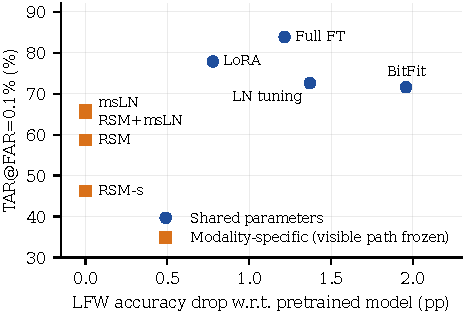
\includegraphics[width=\columnwidth]{tradeoff.pdf}
\caption{Thermal-to-visible verification accuracy versus visible-light forgetting (FP32, mean of 15 runs). Modality-specific methods have zero forgetting by construction; shared methods trade LFW accuracy for thermal accuracy.}
\label{fig:tradeoff}
\end{figure}

\subsection{Effect of Head Pose}
The gallery contains frontal visible images only, while thermal probes span nine head positions (Fig.~\ref{fig:poses}). Fig.~\ref{fig:pose} breaks rank-1 accuracy down by probe position (seed 0, five folds). Without adaptation, accuracy varies between 27.7\% (position 9) and 40.5\% (position 2), but it is low everywhere, so the modality gap rather than pose is the dominant difficulty. After adaptation, accuracy is nearly uniform across positions: 93.2--97.3\% for full fine-tuning and 87.0--97.2\% for msLN. Position 6 is the hardest for every adapted model, and positions 7 and 8 are among the easiest.

\begin{figure}[t]
\centering
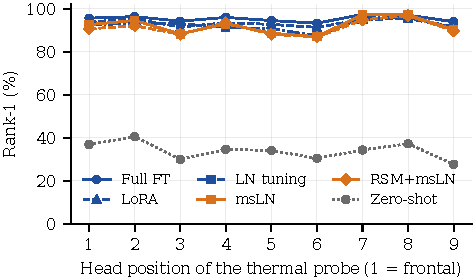
\includegraphics[width=\columnwidth]{pose.pdf}
\caption{Thermal-to-visible rank-1 accuracy per head position of the probe (FP32, seed 0, mean over five folds). The gallery contains frontal visible images only.}
\label{fig:pose}
\end{figure}


\subsection{Quantization Is Modality-Asymmetric}
\label{sec:asym}
Fig.~\ref{fig:int8drop} compares, for the same models, the rank-1 accuracy lost to INT8 quantization for thermal and for visible probes. For visible probes the loss is negligible (at most 0.3\,pp). For thermal probes it ranges from 2.2\,pp (full fine-tuning) to 13.7\,pp (RSM-s), and even the unadapted model loses 5.1\,pp. Quantization noise that is harmless for well-separated visible embeddings is thus significant for thermal embeddings, which lie much closer to the decision boundary (Section~\ref{sec:scores}).

The loss also grows as fewer parameters are adapted: 2.2\,pp for full fine-tuning, 3.0--7.4\,pp for the methods with 5--20\,k parameters, and 13.7\,pp for the 2.7\,k-parameter RSM-s. A plausible explanation is that full fine-tuning can reshape the whole network so that thermal embeddings become well separated, whereas methods that modulate a frozen network rely on small, precise feature shifts that quantization noise can overwhelm. Among the modality-specific methods, adding RSM to msLN reduces the INT8 loss from \pmstd{7.4}{2.5} to \pmstd{5.0}{1.7}\,pp and gives the best quantized accuracy without forgetting (86.2\% rank-1, 54.4\% TAR@0.1\%).

\begin{figure}[t]
\centering
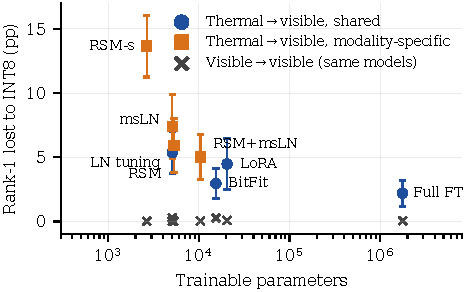
\includegraphics[width=\columnwidth]{int8_drop.pdf}
\caption{Rank-1 accuracy lost to full dynamic INT8 quantization (FP32 minus INT8, mean $\pm$ standard deviation of 15 paired runs) versus the number of trainable parameters. Crosses show the loss for visible probes of the same models, which never exceeds 0.3\,pp.}
\label{fig:int8drop}
\end{figure}

\subsection{Score Distributions}
\label{sec:scores}
Fig.~\ref{fig:scores} shows the distributions of cosine similarity between thermal probes and visible templates (seed 0, all folds pooled). Without adaptation, genuine pairs score only 0.145 on average against 0.012 for impostor pairs (decidability $d'=1.39$). Adaptation mainly raises the genuine scores, to 0.486 for full fine-tuning ($d'=4.11$) and 0.355 for msLN ($d'=3.33$), while the impostor distribution stays centered at zero. The modality-specific methods therefore separate the two classes with a smaller margin, which is consistent with their lower TAR at strict FAR. INT8 quantization leaves the impostor distribution essentially unchanged (mean shift ${\le}0.015$) but moves the genuine distribution toward it, by 0.030 for full fine-tuning, 0.044 for msLN, and 0.049 for LoRA, reducing $d'$ to 3.80 and 2.92 for full fine-tuning and msLN, respectively. Quantization thus erodes exactly the margin that adaptation has built, and the smaller that margin, the more identification errors it causes.

\begin{figure*}[t]
\centering
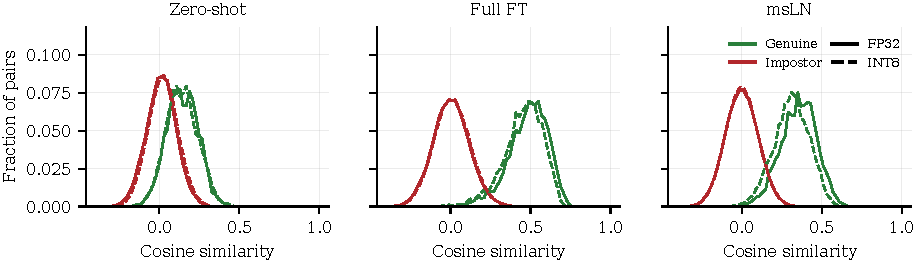
\includegraphics[width=\textwidth]{scores.pdf}
\caption{Distributions of thermal-probe--visible-template cosine similarity for genuine and impostor pairs (seed 0, five folds pooled), in FP32 (solid) and with all linear layers in INT8 (dashed). Quantization shifts genuine scores toward the impostor distribution, which itself is unaffected.}
\label{fig:scores}
\end{figure*}


\subsection{Where the Quantization Loss Comes From}
To locate the loss, the linear layers of only some stages are quantized (Table~\ref{tab:mixed} and Fig.~\ref{fig:stage}). Quantizing stages 1--3, which hold 44\% of the linear-layer weights, reproduces almost the whole INT8 loss, whereas quantizing only stage~4, which holds 51\%, costs between $-0.01$ and 1.2\,pp of rank-1 accuracy relative to FP32 for every method. Sensitivity is therefore far from proportional to parameter count: the stage with the most weights is the least sensitive.

Quantizing one stage at a time (Fig.~\ref{fig:stage}; seed 0, five folds) identifies stage~3 as the main source of the loss: on its own it costs 1.3\,pp of rank-1 accuracy for full fine-tuning and 2.8--4.7\,pp for the parameter-efficient methods, whereas stages 1, 2, and 4 each cost about 1\,pp or less. Stage~3 contains 20 of the 43 factorized layers and operates at $7\times7$ resolution. In five of the six models, the single-stage losses add up to less than the loss of full INT8, indicating that errors introduced in different stages compound as they propagate through the network.


\begin{table*}[t]
\centering
\caption{Mixed-Precision INT8: Thermal-to-Visible Rank-1 / TAR@0.1\% (\%) When Only Some Stages' Linear Layers Are Quantized (5 Folds $\times$ 3 Seeds). Sizes Are for the Serialized EdgeFace-XS Model.}
\label{tab:mixed}
\begin{tabular}{lcccc}
\toprule
 & FP32 & INT8 stage 4 only & INT8 stages 1--3 only & INT8 all \\
 & (6.85\,MB) & (4.59\,MB) & (4.95\,MB) & (2.45\,MB) \\
\midrule
Zero-shot & 33.96 / 6.32 & 33.08 / 6.06 & 30.15 / 5.61 & 28.83 / 5.19 \\
Full fine-tuning & 95.58 / 83.83 & \textbf{95.58} / \textbf{82.82} & 93.53 / 77.10 & 93.38 / 76.70 \\
LoRA & 93.58 / 77.84 & 93.07 / 76.28 & 89.86 / 66.78 & 89.10 / 64.20 \\
BitFit & 92.85 / 71.57 & 92.55 / 70.83 & 90.39 / 66.22 & 89.90 / 64.35 \\
LN tuning & 92.31 / 72.56 & 91.48 / 71.02 & 87.74 / 60.50 & 86.96 / 58.54 \\
msLN & 92.05 / 66.06 & 90.88 / 63.98 & 85.85 / 52.87 & 84.66 / 50.81 \\
RSM+msLN & 91.25 / 65.36 & 90.27 / 63.23 & 86.89 / 57.25 & 86.22 / 54.43 \\
RSM & 88.37 / 58.64 & 87.35 / 56.21 & 83.37 / 47.94 & 82.45 / 44.51 \\
RSM-s & 84.10 / 46.22 & 83.05 / 44.06 & 71.81 / 31.27 & 70.43 / 28.66 \\
\bottomrule
\end{tabular}
\end{table*}

\begin{figure}[t]
\centering
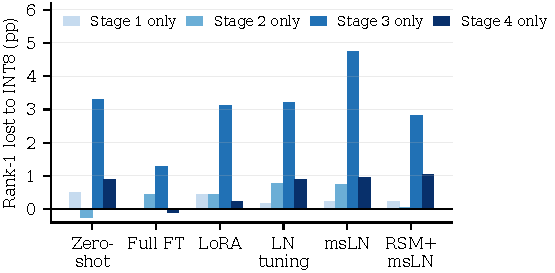
\includegraphics[width=\columnwidth]{stage_int8.pdf}
\caption{Thermal-to-visible rank-1 accuracy lost when the linear layers of a single stage are quantized to INT8 and all other layers stay in FP32 (seed 0, mean over five folds). Stage~3 accounts for most of the loss of every method.}
\label{fig:stage}
\end{figure}

\subsection{Size and Latency}
Table~\ref{tab:latency} reports CPU latency and model size. On this x86 CPU, dynamic INT8 is \emph{slower} than FP32 for both EdgeFace-XS (7.96 vs.\ 6.14\,ms with one thread) and EdgeFace-S (9.29 vs.\ 7.96\,ms). The factorized layers have small inner dimensions, so the cost of quantizing activations at run time and the extra kernel calls outweigh the savings in arithmetic. Quantizing only stage~4 is the fastest quantized configuration (6.53\,ms, 6\% slower than FP32) and reduces the model size by 33\%, while keeping accuracy within 1.2\,pp of FP32 (Table~\ref{tab:mixed}). Full INT8 gives the largest size reduction ($2.8\times$), which matters when storage or memory bandwidth rather than computation is the bottleneck.

\begin{table}[t]
\centering
\caption{Serialized Size and Median CPU Latency per $112\times112$ Face (Intel Xeon Platinum 8470, PyTorch 2.4, Dynamic INT8 With fbgemm)}
\label{tab:latency}
\setlength{\tabcolsep}{4pt}
\begin{tabular}{llccc}
\toprule
 & & Size & \multicolumn{2}{c}{Latency (ms)} \\
\cmidrule(lr){4-5}
Model & Precision & (MB) & 1 thread & 4 threads \\
\midrule
\multirow{4}{*}{XS} & FP32 & 6.85 & \textbf{6.14} & \textbf{5.23} \\
 & INT8 stage 4 & 4.59 & 6.53 & 5.70 \\
 & INT8 stages 1--3 & 4.95 & 7.92 & 7.04 \\
 & INT8 all & \textbf{2.45} & 7.96 & 7.24 \\
\midrule
\multirow{4}{*}{S} & FP32 & 14.03 & \textbf{7.96} & \textbf{6.24} \\
 & INT8 stage 4 & 9.28 & 8.10 & 6.59 \\
 & INT8 stages 1--3 & 9.99 & 9.66 & 7.90 \\
 & INT8 all & \textbf{4.89} & 9.29 & 8.11 \\
\bottomrule
\end{tabular}
\end{table}

%=====================================================================
\section{Discussion}
\label{sec:discussion}
%=====================================================================
\subsection{Recommendations for Deployment}
The results suggest a simple decision procedure for a lightweight model that must recognize both visible and thermal probes.
\begin{itemize}
\item If a separate thermal model can be stored and a small loss of visible accuracy is acceptable, \emph{full fine-tuning} is the most accurate choice and the most robust to quantization.
\item If one model must serve both modalities with no visible-light regression, \emph{modality-specific LayerNorm} is a strong and simple default with 5\,k extra parameters; adding \emph{rank-space modulation} improves its quantized accuracy.
\item For quantized deployment, keep \emph{stages 1--3 in higher precision}, stage~3 above all: quantizing only the last stage recovers almost all of the INT8 loss at a modest cost in size and is the fastest quantized configuration on x86 CPUs.
\item Validate quantized models on the \emph{target modality}: visible-light benchmarks hide quantization losses of up to 13.7\,pp in thermal rank-1 accuracy.
\end{itemize}

\subsection{Negative Results}
In preliminary experiments on the development split (single seed), the modality-specific methods were also trained with quantization-aware training, using a fake-quantization module that reproduces PyTorch's dynamic INT8 to within $10^{-4}$ mean relative error per layer, and with a distillation loss that pulls each thermal embedding toward the pretrained embedding of its registered visible frame. Neither gave consistent gains beyond seed-to-seed variation, so they were not pursued in the full protocol. They are reported so that others need not repeat them, with the caveat that a single development run cannot rule out benefits.

\subsection{Limitations}
The study uses a single dataset of 141 subjects recorded in one laboratory with one thermal camera; absolute numbers will not transfer directly to other sensors or uncontrolled conditions. Each test fold contains 28--29 identities, so rank-1 accuracy is optimistic compared with large-gallery deployments, which is why TAR at a strict FAR is also reported. Learning rates were selected on subjects 81--100, which also appear in test folds of the cross-validation; the selection grid was very small (two values per method) and identical across methods, but this is a mild form of leakage. Only post-training dynamic INT8 with per-tensor scales was studied; static, per-channel, or lower-bit quantization may behave differently. Finally, latency was measured on a server-class x86 CPU; ARM processors and neural accelerators use different INT8 kernels and may show different speed-ups.

\subsection{Ethical Considerations}
Face recognition, and thermal surveillance in particular, raises privacy concerns. This work uses only a public dataset whose participants consented to the release of their recordings under an open license, and the sample images shown are taken from that release. The adaptation methods studied here do not increase the capabilities of FR systems beyond matching across spectra, and the benchmark is intended to support the transparent evaluation of such systems.

%=====================================================================
\section{Conclusion}
\label{sec:conclusion}
%=====================================================================
This paper studied how a face recognition model with fewer than two million parameters can be adapted to thermal-to-visible matching under edge constraints, using a reproducible benchmark built only on openly licensed data. Adaptation closes most of the 66\,pp rank-1 gap, but every method that shares parameters with the visible path forgets visible-light accuracy, while modality-specific methods that keep the visible path intact trail by about 6\,pp in TAR at FAR\,=\,0.1\%. Among the latter, normalization-based adaptation is the most effective, and the rank-space modulation proposed here mainly helps under quantization. INT8 quantization hurts thermal matching much more than visible matching, increasingly so for methods that adapt fewer parameters, and this loss, which erodes the margin between genuine and impostor scores, originates mainly in the third stage, so a simple mixed-precision configuration recovers it. Future work will extend the benchmark to other openly licensed thermal datasets and measure latency on embedded ARM hardware.

\section*{Data and Code Availability}
SpeakingFaces is available under the CC BY 4.0 license at \url{https://huggingface.co/datasets/issai/Speaking_Faces}. The download and alignment pipeline, training and evaluation code, experiment configurations, and per-run results are available at \url{https://github.com/INFUNDER/Face-Recognition-Research}.

\section*{Acknowledgment}
The author thanks the creators of SpeakingFaces for releasing the dataset under an open license, and acknowledges the high-performance computing facility used for the experiments.

\bibliographystyle{IEEEtran}
\bibliography{refs}

\end{document}
